\subsection{Sparse linear algebra}

  \begin{itemize}
    \item Explain format and computation problem (bandwidth, ...)
    \item Allow to solve large problem
  \end{itemize}


Unlike Dense Linear Algebra, computations of Sparse problems are irregular.
%
This is mainly due to the matrix storage format.
%
Indeed, to have an efficiently storage, we only store non-zero values of the matrices.
%
The non-zero pattern of the matrix is define by the problem we tried to resolve.
%
Some storage format are optimized for some class of problem, but there is also very generic format.
%
One of the most generic format is COO\ref{fig:COO}.
%
In COO format, one can store all non-zero elements with their 2D coordinates.
%
Another well use format is CSR\ref{fig:CSR} (Compress Sparse Row) where all non zeros are sorted by row.
%
The row id of a non zero value is then obtain thanks an array.

\begin{figure}[!ht]
     \begin{center}
        \subfigure[Sparse matrix example]{%
            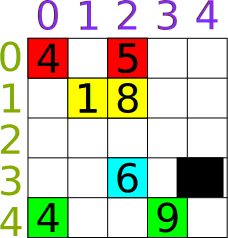
\includegraphics[width=0.25\textwidth]{matrix_format}
        }%
        \subfigure[COO storage]{%
           \label{fig:COO}
           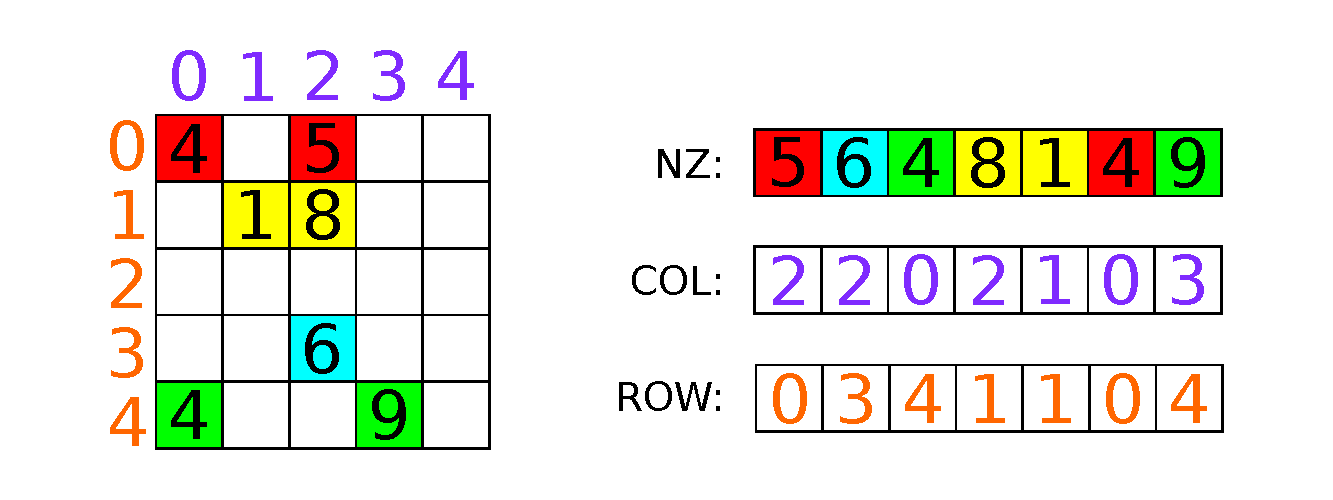
\includegraphics[width=0.35\textwidth]{COO}
        }%
        \subfigure[CSR storage]{%
            \label{fig:CSR}
            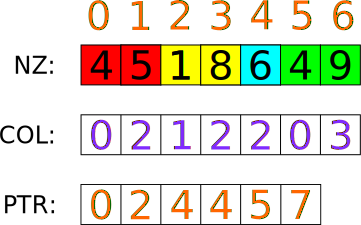
\includegraphics[width=0.35\textwidth]{CSR}
        }%
    \end{center}
    \caption{Comparison between COO and CSR matrix format storage.}
    \label{fig:matrix_storage}
\end{figure}

The choice of the storage format has a lot of impact over the performance of an application.
%
With most of format, we will have to do at least two memory access to obtain 2D coordo ate of a non zero element whereas in dense algebra it could be calculate from the position in the matrix.
%
The sparsity and irregularity of matrices also imply to have unnefficient in memory sparse kernel because of bad cache reuse.
